\hammerpage%

\frame{%
    \centering
    \begin{figure}
        
\includegraphics[width=.8\textwidth]{img/gorilla.png}
        \caption{%
            via: BBC News (\url{%
                https://www.bbc.co.uk/news/technology-33347866
            })
        }
    \end{figure}
}

\frame{%
    \alert{Reliability}
    \begin{itemize}
        \item[] \fullcite{Hyndman2014}
    \end{itemize}

    \alert{Frailty}
    \begin{itemize}
        \item[] \fullcite{Torralba2011}
    \end{itemize}
}

\frame{%
    \centering
    \resizebox{!}{.9\paperheight}{%
        \begin{tikzpicture}

    % Algorithms
    \node[%
        rectangle,
        rounded corners,
        minimum height=2cm,
        minimum width=6cm,
        fill=orange!15,
        label={\Large Algorithms}
    ] (algs) at (0, 0) {};

    % Data
    \node[%
        ellipse,
        minimum height=3cm,
        minimum width=6cm,
        fill=cyan!15,
        label={below:\Large Data}
    ] (data) at (0, -6) {};

    \node[circle, fill=orange, thick, inner sep=2pt, minimum size=2mm]
        (a) at (1, 0) {};
\end{tikzpicture}

    }
}

\section{Generating artificial data}

\frame{%
    \centering
    \begin{figure}
        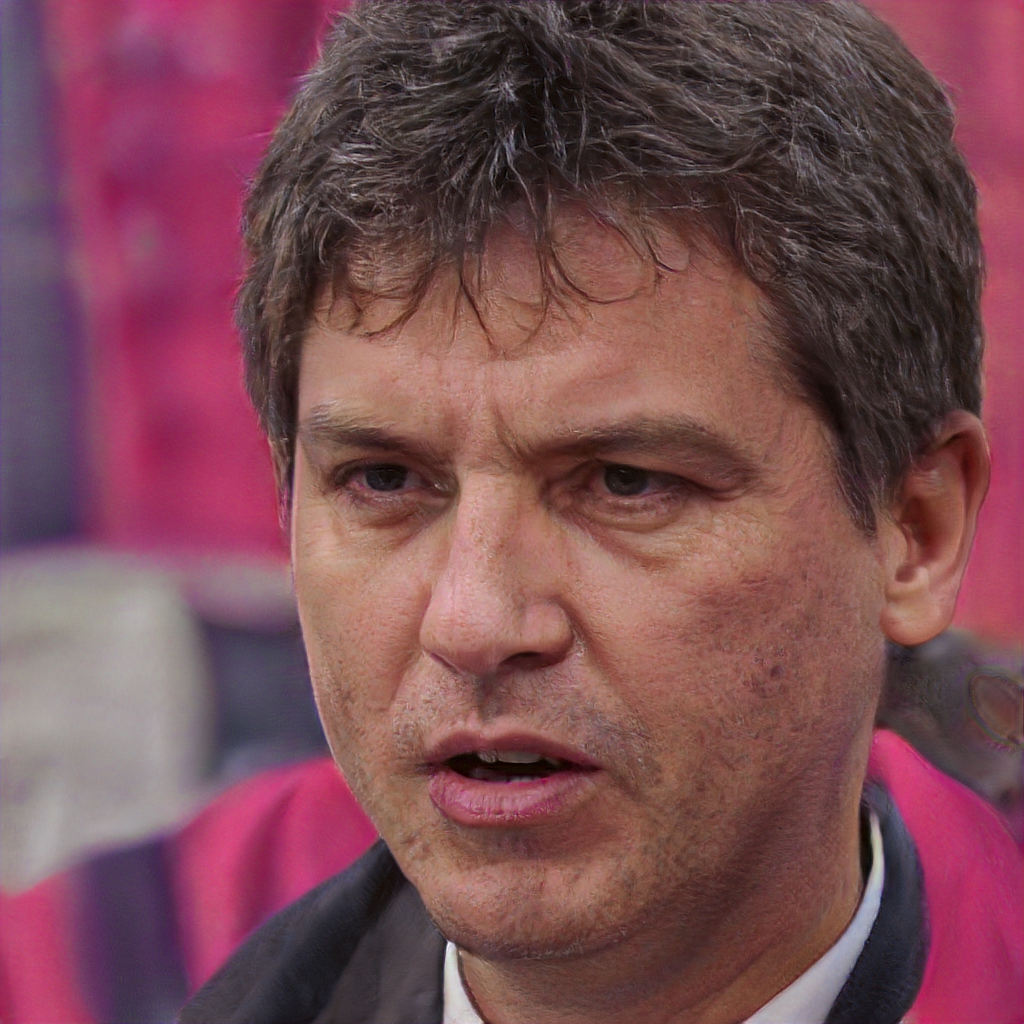
\includegraphics[width=.3\textwidth]{img/faces/0.jpeg}\hfill%
        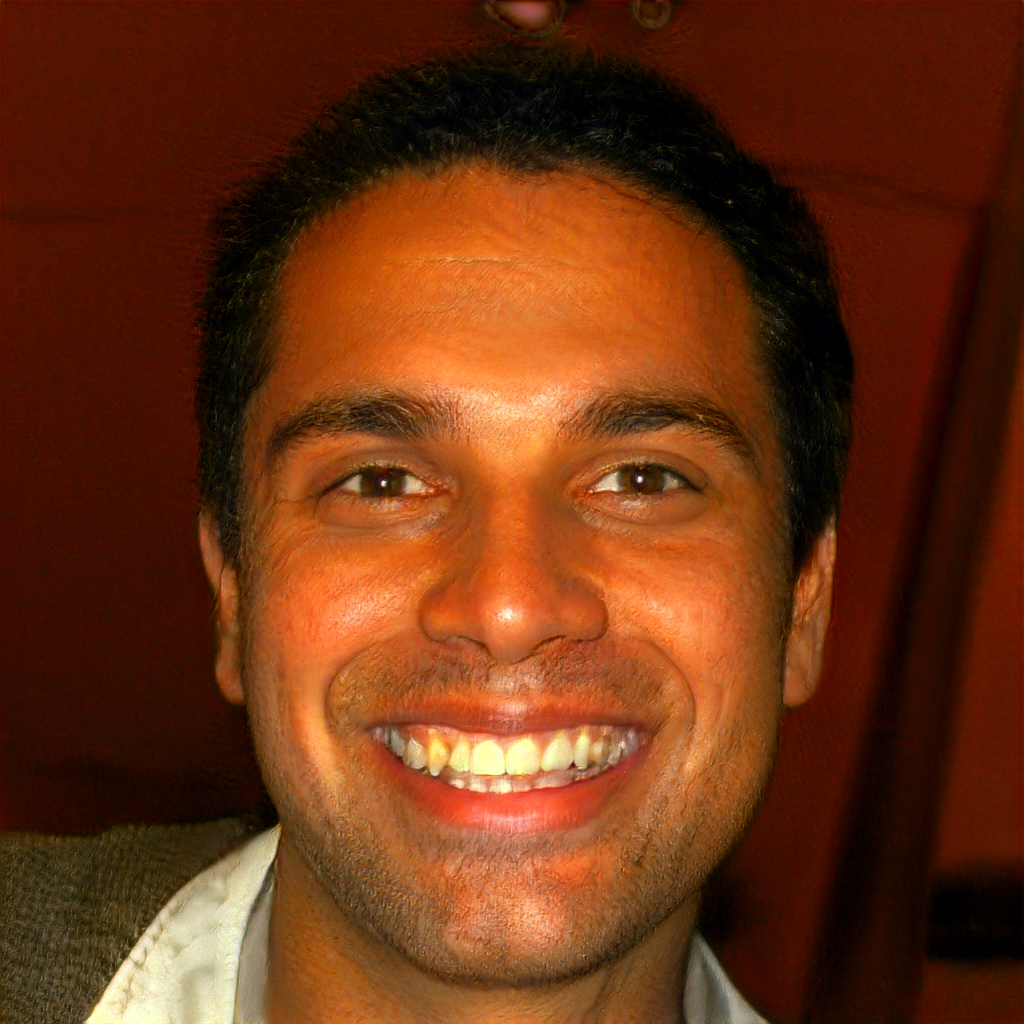
\includegraphics[width=.3\textwidth]{img/faces/1.jpeg}\hfill%
        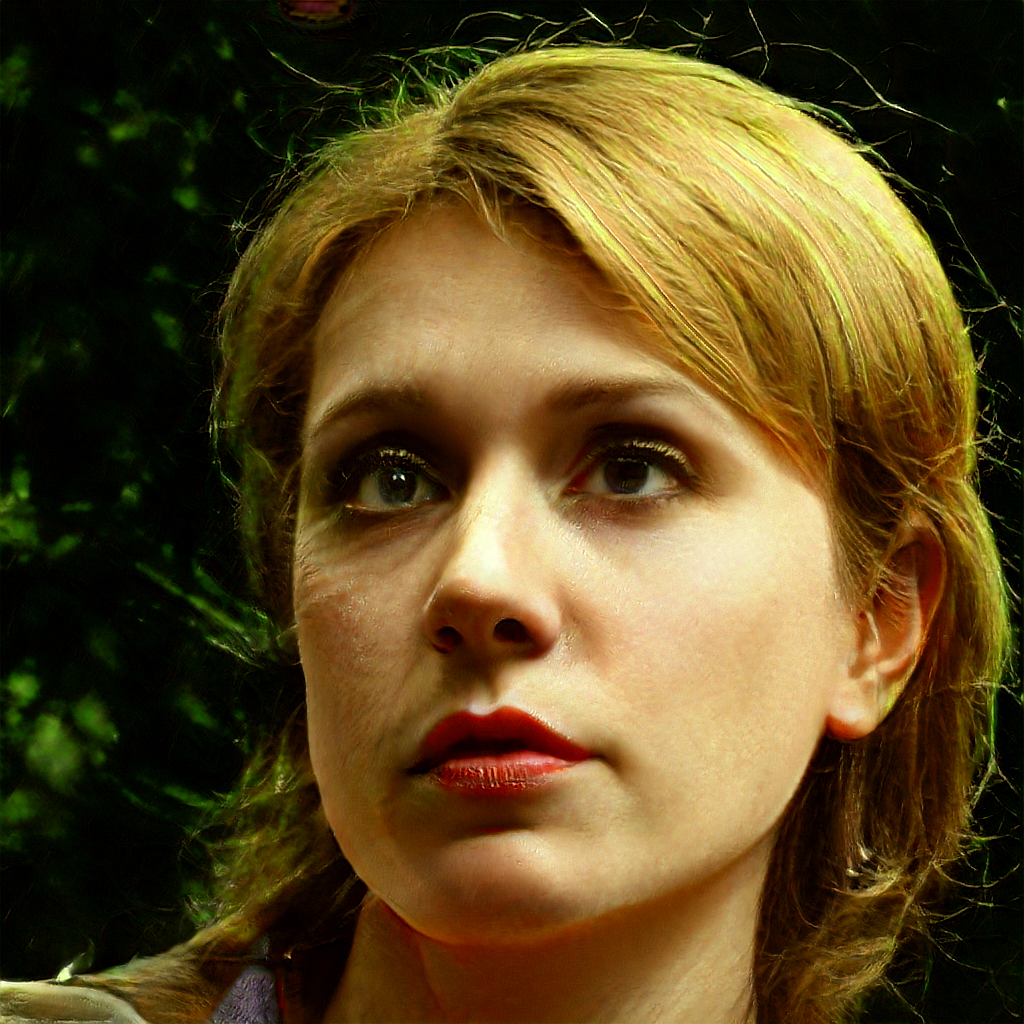
\includegraphics[width=.3\textwidth]{img/faces/2.jpeg}
        \caption{via: \url{https://thispersondoesnotexist.com}}
    \end{figure}
}

\frame{%
    \begin{figure}
        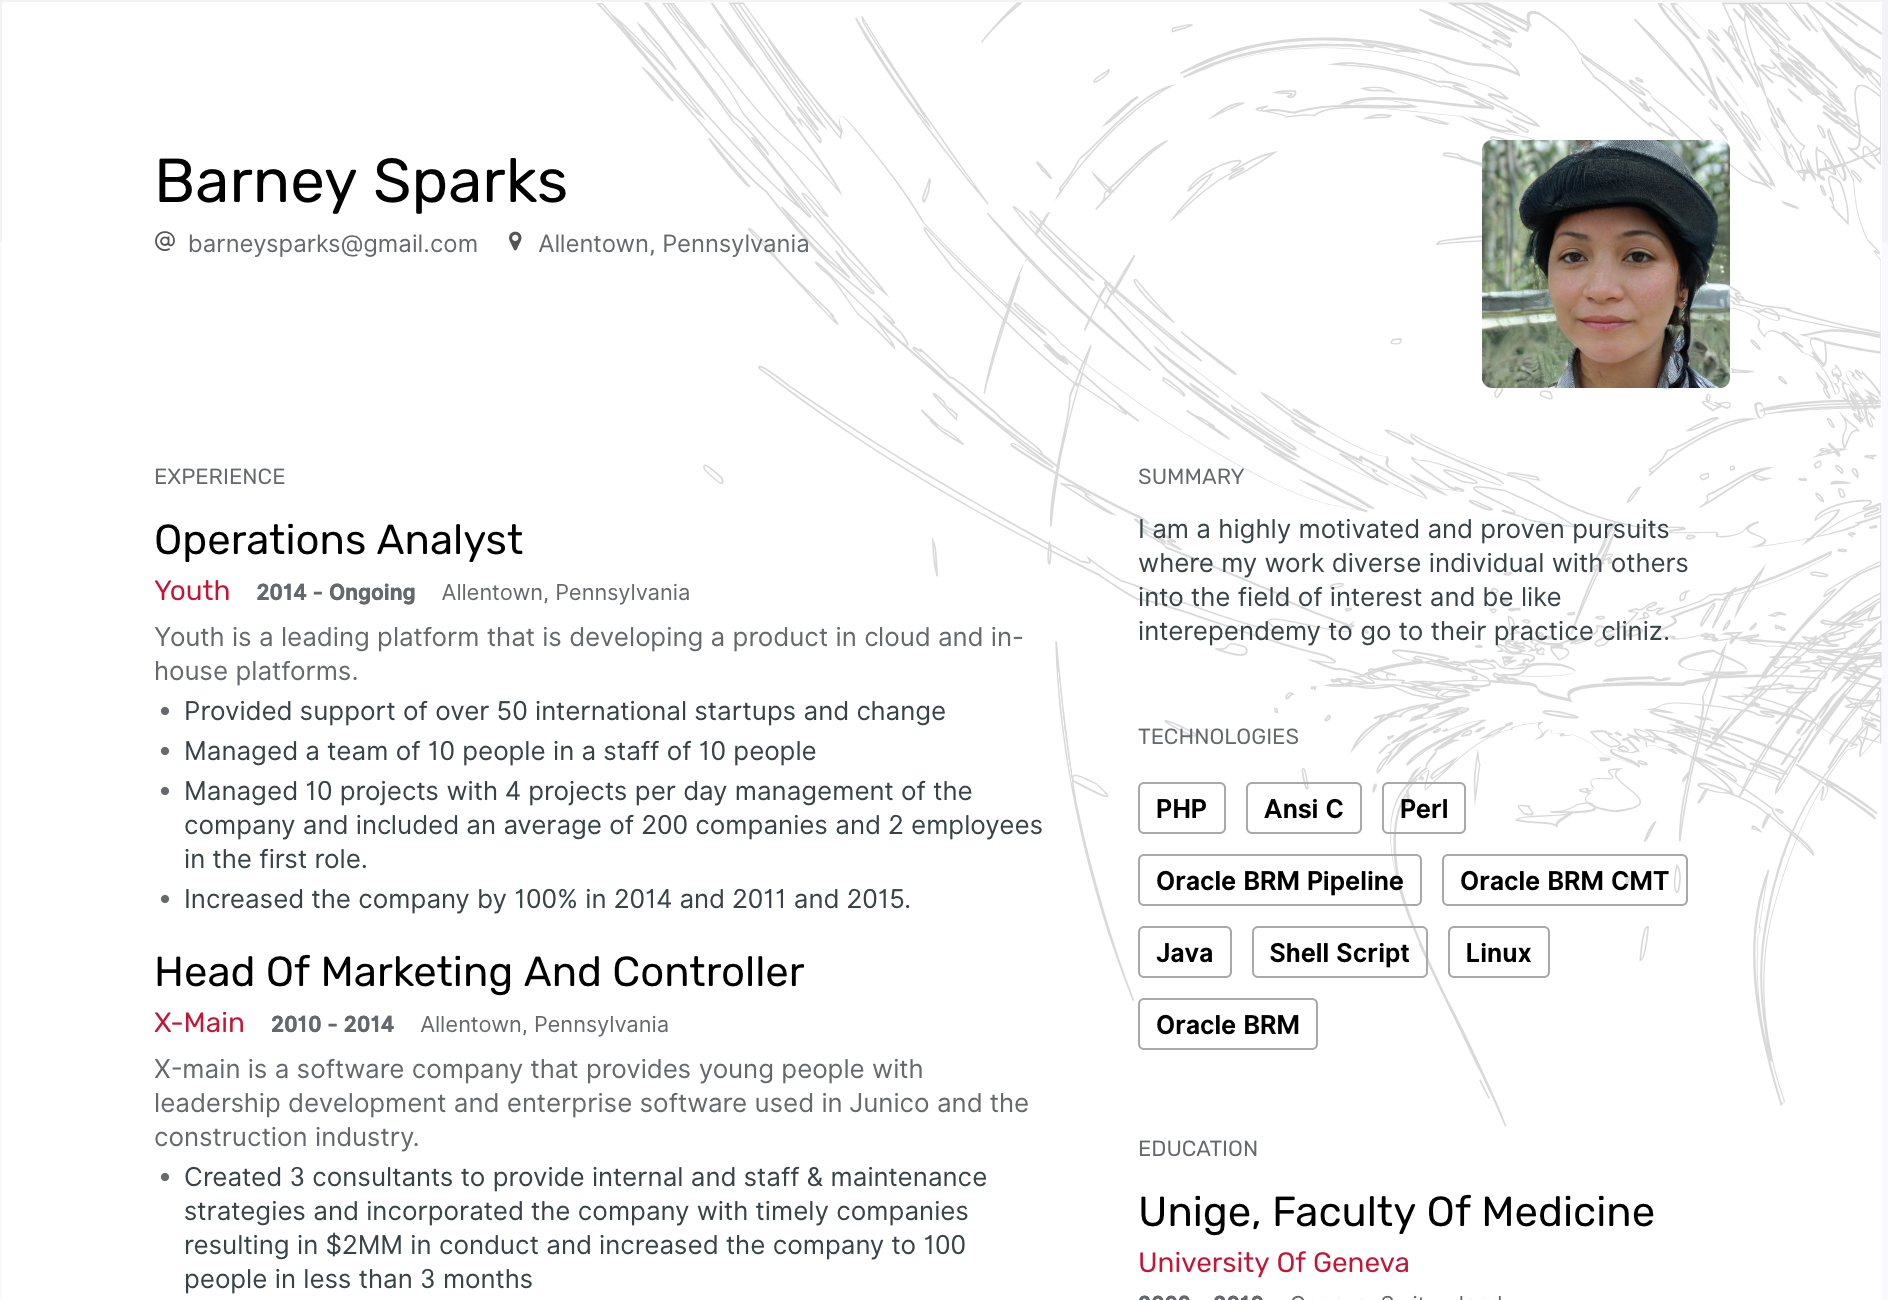
\includegraphics[width=\textwidth]{img/resume.png}
        \caption{via: \url{https://thisresumedoesnotexist.com}}
    \end{figure}
}

\frame{%
    \begin{figure}
        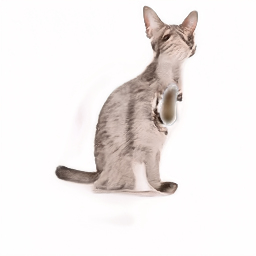
\includegraphics[width=.45\textwidth]{img/cats/0.jpeg}\hfill%
        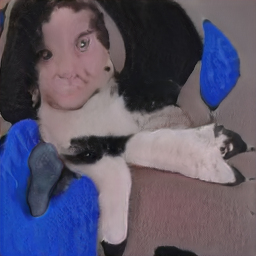
\includegraphics[width=.45\textwidth]{img/cats/1.jpeg}
        \caption{via: \url{https://thiscatdoesnotexist.com}}
    \end{figure}
}

\frame{%
    \alert{Anscombe's quartet}\vfill
    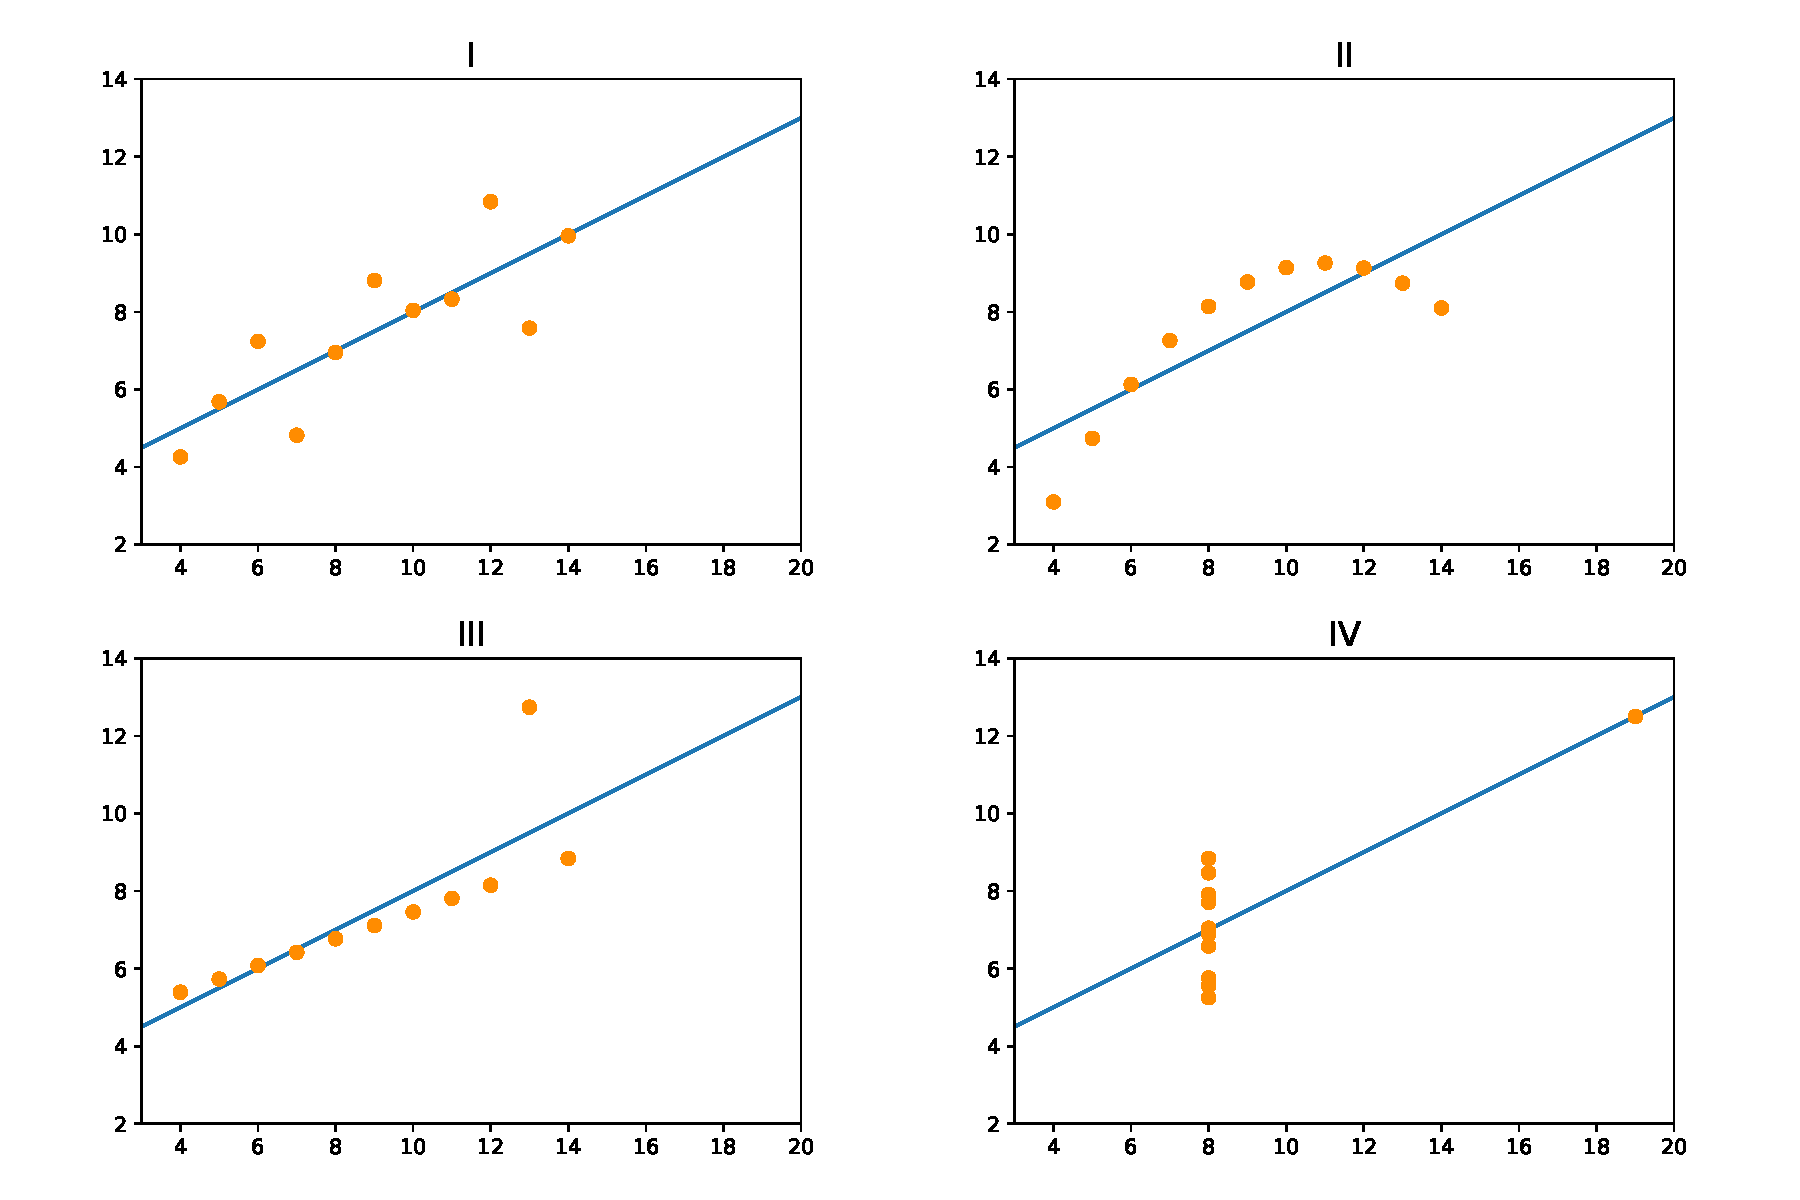
\includegraphics[width=\textwidth]{img/anscombes.pdf}\vfill
}

\frame{%
    \alert{The Datasaurus dozen}\vfill
    \begin{figure}
        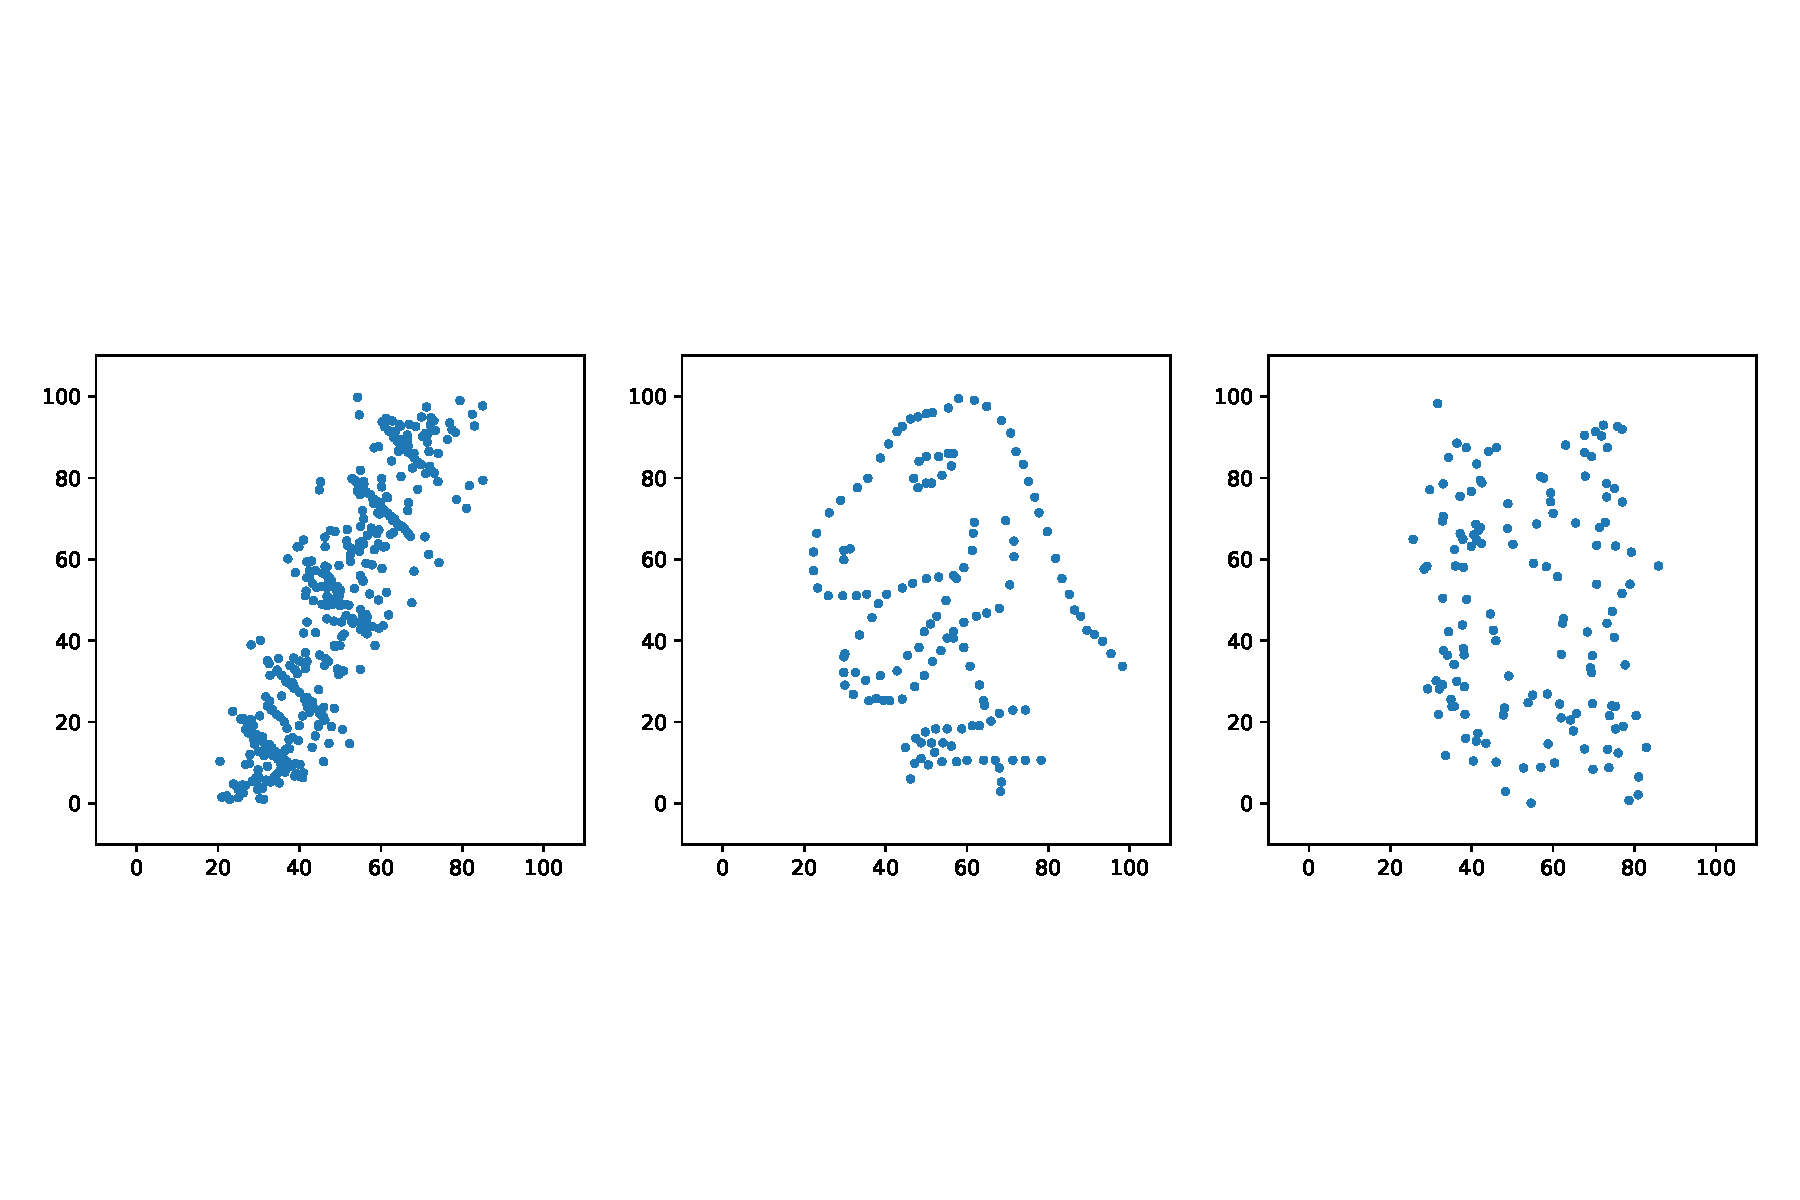
\includegraphics[width=\textwidth]{img/datasaurus.pdf}
        \caption{Original paper by @JustinMatejka}
    \end{figure}\vfill
}

\frame{%
    \resizebox{\textwidth}{!}{%
        \begin{tikzpicture}

    % Dataset
    \fill[gray!15] (-4, 5) rectangle (-2, 8.5);
    \fill[cyan!35] (-2, 5) rectangle (0, 8.5);
    \fill[magenta!5] (0, 5) rectangle (2, 8.5);
    \path (-2, 5) pic {fullcolumn=10}
          (0, 5) pic {fullcolumn=10}
          (2, 5) pic {fullcolumn=10};
    \node (dataset) at (-1, 4.5) {};

    % A similar dataset
    \pause%
    \fill[pattern=north west lines, pattern color=cyan!35]
        (6, 0) rectangle (8, 3.15);
    \fill[pattern=north east lines, pattern color=magenta!50]
        (8, 0) rectangle (10, 3.15);
    \fill[pattern=north west lines, pattern color=gray!50]
        (10, 0) rectangle (12, 3.15);
    \path (8, 0) pic {fullcolumn=9}
        (10, 0) pic {fullcolumn=9}
        (12, 0) pic {fullcolumn=9};
    \node (similar) at (5.5, 2) {};

    \pause%
    \draw[orange, ultra thick, rounded corners]
        (-4.5, 4.4) rectangle (2.5, 9.2);
    \draw[->, orange, ultra thick]
        (dataset.south) to [out=290, in=180] (similar.west)
        node[midway, above=10pt] {\Large\color{orange} make `similar'};

\end{tikzpicture}

    }
}

\frame{%
    \huge{%
        Given an algorithm, how can one find sets of data for which it performs
        well?
    }
}

